% Paquets généraux
\documentclass[a4paper,12pt,titlepage,twoside]{article}
\usepackage[T1]{fontenc}
\usepackage[utf8]{inputenc}
\usepackage[french]{babel}
\usepackage{subcaption}
\addto\captionsfrench{%
  \renewcommand{\tablename}{Tableau}%
}
\usepackage[gen]{eurosym}
%\usepackage[dvips]{graphicx}
\usepackage{minted}
\usepackage{fancyhdr}
\usepackage{pdfpages} 
\usepackage{multido}
\usepackage{hyperref}
\usepackage{textcomp}
\usepackage{schemabloc}
%\usepackage[bitstream-charter]{mathdesign}
\usepackage{array}
\newcolumntype{P}[1]{>{\centering\arraybackslash}p{#1}}
\usepackage[shortlabels]{enumitem}
\usepackage[framemethod=TikZ]{mdframed}

\newcommand{\id}{71}
\newcommand{\nom}{Théorie des mécanismes}
\newcommand{\sequence}{04}
\newcommand{\nomsequence}{Liaisons entre les solides}
\newcommand{\num}{02}
\newcommand{\type}{KH}
\newcommand{\descrip}{Liaisons équivalentes, hyperstatisme, liaisons en série et en parallèle, théorie des graphes}
\newcommand{\competences}{B2-12: Proposer une modélisation des liaisons avec leurs caractéristiques géométriques. \\ &  B2-13: Proposer un modèle cinématique paramétré à partir d'un système réel, d'une maquette numérique ou d'u \\ &  B2-17: Simplifier un modèle de mécanisme. \\ &  B2-18: Modifier un modèle pour le rendre isostatique. \\ &  C1-04: Proposer une démarche permettant d'obtenir une loi entrée-sortie géométrique.  \\ &  C2-05: Caractériser le mouvement d'un repère par rapport à un autre repère. \\ &  C2-06: Déterminer les relations entre les grandeurs géométriques ou cinématiques. }
\newcommand{\nbcomp}{7}
\newcommand{\systemes}{}
\newcommand{\systemesnum}{}
\newcommand{\systemessansaccent}{}
\newcommand{\ilot}{2}
\newcommand{\ilotstr}{02}
\newcommand{\dossierilot}{\detokenize{Ilot_02 }}

%\usepackage{style}
\usepackage{bodegraph}
\usepackage{rpcinematik}
\usepackage[locale = FR]{siunitx}
\usepackage{caption}
\newcommand{\institute}{Lycée Dorian}

\usepackage{listings}
\usepackage{fancyvrb}
\usepackage{color}
\usepackage{xcolor}
\usepackage{colortbl}
\usepackage{helvet}
\usepackage[frenchmath]{newtxsf} % for sans serif symbols
\renewcommand{\familydefault}{\sfdefault}
%\usepackage{amsfonts}
%\usepackage{amsmath}
%\usepackage{lmodern}
\usepackage{mathastext}
%\usepackage{xspace}
\usepackage{varioref}
\usepackage{tabularx}
%\usepackage{floatflt}
\usepackage{graphics}
\usepackage{wrapfig}
\usepackage{textcomp}
\usepackage{tikz,tkz-tab}
\usepackage[european resistor, european voltage, european current]{circuitikz}
\usepackage{wrapfig}
\usepackage{gensymb}
\usepackage[percent]{overpic}
\usetikzlibrary{babel}
\usepackage{ifthen}
\usepackage{cancel}
\usepackage{etoolbox}
\usepackage{multirow}
%\usepackage{boxedminipage}
\definecolor{gris25}{gray}{0.75}
\definecolor{bleu}{RGB}{18,33,98}
\definecolor{bleuf}{RGB}{42,94,171}
\definecolor{bleuc}{RGB}{231,239,247}
\definecolor{bleum}{RGB}{160,195,226}
\definecolor{rougef}{RGB}{185,18,27}
\definecolor{rougec}{RGB}{255,188,204}%255,230,231
\definecolor{vertf}{RGB}{103,126,82}
\definecolor{vertc}{RGB}{220,255,191}
\definecolor{forestgreen}{rgb}{0.13,0.54,0.13}
\definecolor{blcr}{rgb}{0.59,0.69,0.84}
\definecolor{blfr}{rgb}{0.32,0.51,0.75}
\definecolor{orfr}{rgb}{0.90,0.42,0.15}
\definecolor{orcr}{rgb}{0.90,0.65,0.50}
\definecolor{orangef}{rgb}{0.659,0.269,0.072}
\definecolor{orange}{rgb}{0.58,0.35,0.063}
\definecolor{orangec}{rgb}{0.43,0.32,0.25}
\definecolor{rcorrect}{rgb}{0.6,0,0}
\definecolor{sequence}{rgb}{0.75,0.75,0.75}
\definecolor{competences}{rgb}{0.61,0.73,0.35}
\definecolor{rose}{HTML}{ff00ff}
\definecolor{grisf}{HTML}{222222}
\definecolor{grisc}{HTML}{636363}
\definecolor{normal}{HTML}{4087c4}
\definecolor{info}{HTML}{5bc0de}
\definecolor{success}{RGB}{92,184,92}
\definecolor{warning}{RGB}{240,173,78}
\definecolor{danger}{RGB}{217,83,79}
\hypersetup{                    % parametrage des hyperliens
    colorlinks=true,                % colorise les liens
    breaklinks=true,                % permet les retours à la ligne pour les liens trop longs
    urlcolor= blfr,                 % couleur des hyperliens
    linkcolor= orange,                % couleur des liens internes aux documents (index, figures, tableaux, equations,...)
    citecolor= forestgreen                % couleur des liens vers les references bibliographiques
    }

\newcolumntype{M}[1]{>{\centering\arraybackslash}m{#1}}
\definecolor{codegreen}{rgb}{0,0.6,0}
\definecolor{codegray}{rgb}{0.5,0.5,0.5}
\definecolor{codepurple}{rgb}{0.58,0,0.82}
\definecolor{backcolour}{rgb}{0.95,0.95,0.92}

\lstdefinestyle{mystyle}{
    backgroundcolor=\color{backcolour},   
    commentstyle=\color{codegreen},
    keywordstyle=\color{magenta},
    numberstyle=\tiny\color{codegray},
    stringstyle=\color{codepurple},
    basicstyle=\ttfamily\footnotesize,
    breakatwhitespace=false,         
    breaklines=true,                 
    captionpos=b,                    
    keepspaces=true,                 
    numbers=left,                    
    numbersep=5pt,                  
    showspaces=false,                
    showstringspaces=false,
    showtabs=false,                  
    tabsize=2
}

\lstset{style=mystyle}

% Mise en page
\pagestyle{fancy}

\setlength{\hoffset}{-18pt}
\setlength{\oddsidemargin}{0pt} 	% Marge gauche sur pages impaire2s
\setlength{\evensidemargin}{0pt} 	% Marge gauche sur pages paires
\setlength{\marginparwidth}{00pt} 	% Largeur de note dans la marge
\setlength{\headwidth}{481pt} 	 	% Largeur de la zone de tête (17cm)
\setlength{\textwidth}{481pt} 	 	% Largeu\textbf{r de la zone de texte (17cm)
\setlength{\voffset}{-18pt} 		% Bon pour DOS
\setlength{\marginparsep}{7pt}	 	% Séparation de la marge
\setlength{\topmargin}{-30pt} 		% Pas de marge en haut
\setlength{\headheight}{55pt} 		% Haut de page
\setlength{\headsep}{20pt} 		% Entre le haut de page et le texte
\setlength{\footskip}{30pt} 		% Bas de\textbf{ page + séparation
\setlength{\textheight}{700pt} 		% Hauteur de l'icone zone de texte (25cm)
\setlength\fboxrule{1 pt}
\renewcommand{\baselinestretch}{1}
\setcounter{tocdepth}{1}
\newcommand{\cadre}[2]
{\fbox{
  \begin{minipage}{#1\linewidth}
   \begin{center}
    #2\\
   \end{center}
  \end{minipage}
 }
}

\newcommand{\repon}[1]
{
~\ \\
\begin{tabular}{|m{\linewidth}|}
 \hline
\multido{}{#1}{\\ \hline}
\end{tabular}
}


\newcommand{\objectif}[1]{
\mdfsetup{%
frametitle={%
\tikz[baseline=(current bounding box.east),outer sep=0pt]
\node[anchor=east,rectangle,fill=bleum]
{\strut Objectif~};}}
\mdfsetup{innertopmargin=10pt,linecolor=bleum,%
linewidth=2pt,topline=true,%
frametitleaboveskip=\dimexpr-\ht\strutbox\relax
}
\begin{mdframed}[]\relax%
#1
\end{mdframed}}


\newcounter{num_quest} \setcounter{num_quest}{0}
\newcounter{num_rep} \setcounter{num_rep}{0}
\newcounter{num_cor} \setcounter{num_cor}{0}

\newcommand{\feuilleDR}[1]{
	\begin{tikzpicture}
		\draw[gray!30](0,0)grid[step=0.5cm](\linewidth,#1);
	\end{tikzpicture}
}

%\newcommand{\question}[1]{\refstepcounter{num_quest}\par
%~\ \\ \parbox[t][][t]{0.15\linewidth}{\textbf{Question \arabic{num_quest}}}\parbox[t][][t]{0.85\linewidth}{#1\label{q\the\value{num_quest}}}\par
%}

\newcommand{\question}[1]{\refstepcounter{num_quest}\par
~\ \\ \textbf{Question \arabic{num_quest} : }#1\label{q\the\value{num_quest}}\par
}

\newcommand{\posetafigure}[3]{
\begin{figure}[ht!]
 \begin{center}
  \includegraphics[width=#2\linewidth]{img/#1}
 \end{center}
 \caption{\label{#1} #3}
\end{figure}}

\newcommand{\goforum}{
\begin{figure}

\end{figure}
\begin{center}
 
\includegraphics[width=0.7\linewidth]{../../../img/go_forum}
\end{center}
\label{go_forum}
\caption{J'pète les plombs}
\end{figure}}

\newcommand{\reponse}[4][1]
{\noindent
\parbox{\textwidth}{
\rule{\linewidth}{.5pt}\\
\textbf{Question\ifthenelse{#1>1}{s}{} \multido{}{#1}{%
\refstepcounter{num_rep}\ref{q\the\value{num_rep}} }:} ~\ \\
\ifdef{\public}{#3 \ifthenelse{#2>0}{~\ \\ 	\feuilleDR{#2}}}{#4}
}}

\newcommand{\cor}
{\refstepcounter{num_cor}
\noindent
\rule{\linewidth}{.5pt}
\textbf{Question \arabic{num_cor}:} \\
}

\newcommand{\finsujet}
{
    \begin{center}
    \Large{FIN}
    \end{center}

    \cleardoublepage

    \ifdef{\public}{\pagestyle{docreponse}}{\pagestyle{correction}}

    \ifdef{\public}{
        \begin{tikzpicture} 
            \draw (0,0) rectangle (2,2);
            \draw (0,0) -- (2,2);
            \draw (1.5,0.5) node {\large 20};
            \draw (2.5,0) rectangle (16,2);
            \draw (4.5,1.7) node {\large Commentaires:};
        \end{tikzpicture}
    }
    ~\ \\
}


%\newcommand{\repcarre}[2]
%{
%~\ \\
%\begin{tikzpicture}
%\draw [fill=white] (0,0) rectangle +(\linewidth,#1);
%\node[align=left] at (1.1,#2-0.3) {\textbf{Question #1:}};
%\end{tikzpicture}
%}

\newcommand{\titre}[1]
{\begin{center}
\cadre{0.8}{\huge #1} 
\end{center}
}


%Définition des torseurs :
\newcommand{\torseur}[2]{\left\{\mathcal{#1}_{#2} \right\}}
\newcommand{\torseurh}[3]{\left\{\genfrac{}{}{0pt}{0}{#1}{#2}\right\}_{#3}}
\newcommand{\torseurv}[8]{\left\{
\begin{matrix}
#1 & #4 \\ #2 & #5 \\ #3 &#6
\end{matrix}
\right\}_{{#7},{#8}}}

%Définition des torseurs :
%\newcommand{\torseur}[2]{\left \{\mbox{\relsize{2}{$\mathcal {#1}$}\relsize{-2}}\phantom{}_{\mbox{\scriptsize $#2$}} \right \}}
%\newcommand{\torseurh}[3]{\left\{\genfrac{}{}{0pt}{0}{#1}{#2}\right\}_{#3}}
%\newcommand{\torseurv}[8]{
%\left\{\begin{array}{@{}c|c@{}} #1 & #4 \\ #2 & #5 \\ #3 & #6 \end{array} \right\}_{#7,#8}
%}
\newcommand{\derivee}[2]{\left.\dfrac{\d #1}{\d t}\right|_{#2}}
\newcommand{\tripleint}{\int\!\!\!\!\!\int\!\!\!\!\!\int}

% Notation cinématique et statique
\newcommand{\cinematique}[2]{\mbox{#1}/\mbox{#2}}
\newcommand{\statique}[2]{\mbox{#1}\rightarrow\mbox{#2}}
\newcommand{\moment}[3]{\vv {#1}_{\scriptsize{#3}}(#2)}
\newcommand{\resultante}[2]{\vv {#1}_{\scriptsize{#2}}}


%Commande de base
\newcommand{\jo}{\left(j\omega\right)} % j \omega dans l'analyse fréquentielle
\newcommand{\tl}{\xrightarrow{\mathcal{L}}} % transformée de laplace sur fleche
\newcommand{\tli}{\xrightarrow{\mathcal{L}^{-1}}} % transformée inverse de laplace sur fleche
\renewcommand{\d}[1][]{\mathrm{d#1}}
\newcommand{\dd}[1][]{\mathrm{d#1}}
\newcommand{\vect}[2]{{#1}\wedge{#2}}
\newcommand{\base}[3]{(\vec #1,\vec #2,\vec #3)}
\newcommand{\vectbase}[4]{{\vphantom{\left| \begin{matrix}
#1\\#2\\#3 \end{matrix} \right|}}_{#4}{\left| \begin{matrix}
#1\\#2\\#3 \end{matrix} \right.}}
%Pour avoir les paragraphes sous la forme I, II, III
\renewcommand{\thesection}{\Roman{section}}
\setcounter{secnumdepth}{3}
\renewcommand{\Frlabelitemii}{$\bullet$}

% En tête et pied de page
\lhead{\nom}
\rhead{
\includegraphics[width=2cm]{../../../img/logo}}
\lfoot{\auteurun,\ \auteurdeux}
\cfoot{Page \thepage}

\fancypagestyle{docreponse}{%
  \fancyhf{}
  \fancyhead[LO]{NOM Prénom: .............................}
  \rhead{
\includegraphics[width=2cm]{../../../img/logo}\hspace{2pt}}
  \ifdef{\auteurdeux}{\lfoot{\auteurun,\ \auteurdeux}}{\lfoot{\auteurun}}
  \rfoot{\nom}
  \lfoot{Document réponse}
  \cfoot{Page \thepage}
   }

\fancypagestyle{correction}{%
  \fancyhf{}
  \lhead{\colorbox{danger}{\begin{minipage}{0.65\paperwidth} \textcolor{white}{\textbf{Correction}} \end{minipage}} }
  \rhead{
\includegraphics[width=2cm]{../../../img/logo}}
  \lfoot{Renaud Costadoat, Françoise Puig}
  \rfoot{\colorbox{danger}{\begin{minipage}{0.4\paperwidth} \begin{flushright}\textcolor{white}{\textbf{Correction}}\end{flushright} \end{minipage}} }}

\fancypagestyle{correctioninfo}{%
  \fancyhf{}
  \lhead{\colorbox{danger}{\begin{minipage}{0.65\paperwidth} \textcolor{white}{\textbf{Correction}} \end{minipage}} }
  \rhead{
\includegraphics[width=2cm]{../../../img/logo}}
  \lfoot{Renaud Costadoat, Juliette Genzmer}
  \rfoot{\colorbox{danger}{\begin{minipage}{0.6\paperwidth} \begin{flushright}\textcolor{white}{\textbf{Correction}}\end{flushright} \end{minipage}} }}

\renewcommand{\footrulewidth}{0.4pt}

\usepackage{eso-pic}
\newcommand{\BackgroundPic}{%
\put(0,0){%
\parbox[b][\paperheight]{\paperwidth}{%
\vfill
\begin{center}
\hspace{0.5cm}\vspace{0.5cm}

\includegraphics[width=\paperwidth,height=\paperheight,%
keepaspectratio]{../../../img/fond3}%
\end{center}
\vfill
}}}

\newcommand{\BackgroundPicdeux}{%
\put(25,-30){%
\parbox[b][\paperheight]{\paperwidth}{%
\vfill
\begin{center}
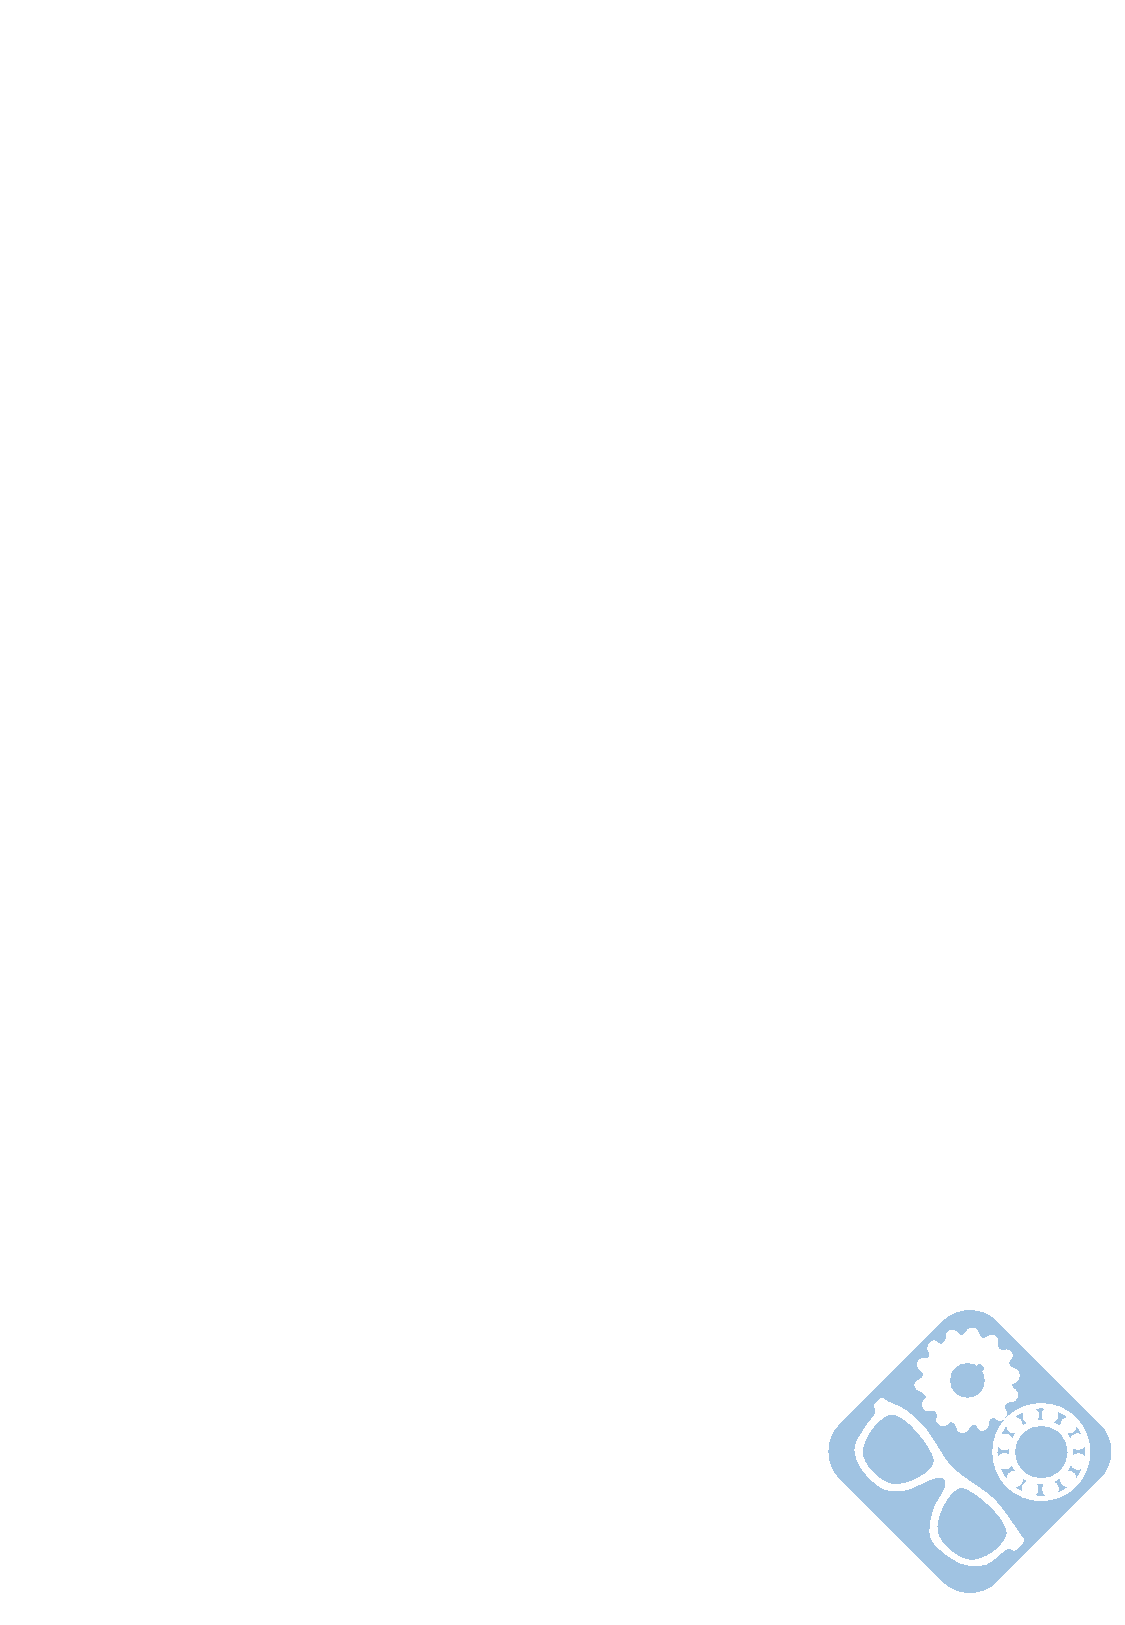
\includegraphics[width=\paperwidth,height=\paperheight,%
keepaspectratio]{../../../img/fond4}%
\end{center}
\vfill
}}}

\begin{document}

\pagestyle{empty}

\AddToShipoutPicture*{\BackgroundPic}


\includegraphics[width=2cm]{../../../img/logo}

\Huge{DS \numero - \sujet}

\vspace{1cm}

\ifdef{\prive}{\begin{center}\colorbox{danger}{\Huge{Avec Correction}}\end{center}}{}

\begin{center}
\centering\huge{PTSI}
\end{center}

\vspace{2cm}


\begin{center}
\centering\Large{\jour}
\end{center}

\vspace{2cm}

\normalsize

\tableofcontents

\newpage

\AddToShipoutPicture{\BackgroundPicdeux}

\pagestyle{fancy}

\begin{center}
\Huge \sujet
\end{center}


\normalsize


\section{Introduction}

La Seine Musicale est un équipement à vocation musicale à fort rayonnement culturel, dont l'objet est de créer ou d'aménager des espaces pour des concerts, des expositions, des installations permanentes ou provisoires.

Conçue par les architectes Shigeru Ban et Jean de Gastines, la Seine Musicale est implantée en pointe aval de l'Ile Seguin à Boulogne-Billancourt, en région parisienne.

L'auditorium, bâtiment principal du projet de la Seine Musicale, est \og posé sur la Seine \fg\ et sa coque en bois semble flotter sur le fleuve, tel un bateau doté d'une voile qui circule autour de l'auditorium en suivant le soleil.

L'un des défis architecturaux de ce projet consiste à mettre en mouvement la voile (figure \ref{fig01}), équipée de 470 panneaux photovoltaïques, autour de l'auditorium, tout en garantissant une acoustique exceptionnelle.

\posetafigure{fig01}{0.8}{Vue de l'auditorium et de la voile}

Afin d'améliorer l'efficacité des panneaux photovoltaïques, le déplacement de la voile s'effectue en suivant l'évolution du soleil au cours d'une journée. La position du soleil (point $C$) par rapport à un point d'observation sur la terre (point $A$) est définie par deux paramètres (figure \ref{fig02}) :
\begin{itemize}
 \item l'élévation $\theta_z$, angle entre la direction d'observation du soleil (droite ($AC$)) et l'horizon (droite ($AB$)) en degrés, avec $\overrightarrow{AC}=r_S\cdot\overrightarrow{x_S}$ et $\overrightarrow{y_H}=\overrightarrow{y_S}$,
 \item l'azimut $\varphi_a$, angle entre la direction ($AB$) et la droite Nord-Sud (Nord : $\varphi_a=0^{\circ}$) avec $\overrightarrow{AC}=r_H\cdot\overrightarrow{x_H}$ et $\overrightarrow{z_T}=\overrightarrow{z_H}$.
\end{itemize}

\newpage

\begin{figure}[ht!]
\begin{center}
   \def\svgwidth{.45\textwidth}
   \input{img/fig02.pdf_tex}
\end{center}
\caption{\label{fig02} Paramétrage de l'azimut et de l'élévation solaires}
\end{figure}

Le déplacement de la voile autour du bâtiment s'effectue périodiquement, toutes les 15 minutes, afin d'éviter que les motorisations soient sollicitées en permanence à des vitesses trop faibles. Les caractéristiques globales que la voile doit respecter lors de ses déplacements sont définies dans l'extrait de cahier des charges fonctionnel présenté tableau \ref{tab01}.

Dans un premier temps, on souhaite s'assurer que le déplacement de la voile respecte les exigences du tableau \ref{tab01}.

\begin{table}[ht!]
\begin{tabular}{|p{0.05\textwidth}|p{0.35\textwidth}|p{0.3\textwidth}|p{0.2\textwidth}|}
\hline
Id & Exigence & Critère & Niveau\\
\hline
1 & La voile doit se déplacer pour suivre le soleil & Période & Toutes les 15 min\\
\hline
1.1 & Le déplacement de la voile doit être imperceptible à l'\oe il humain & Vitesse de déplacement $(\omega_{dep})$ & $\leq 0.18^{\circ}.s^{-1}$ \\
\hline
1.2 & Le déplacement de la voile doit être suffisamment rapide & Temps de déplacement & $<1min$\\
\hline
\end{tabular}
\caption{\label{tab01}Extrait du cahier des charges fonctionnel}
\end{table}

Il est nécessaire pour cela de déterminer le déplacement maximal du soleil durant une période de 15 minutes.

Dans ce but, les évolutions de l'azimut du soleil $\varphi_a$ au cours de la journée sont données en figure \ref{fig03} pour le solstice d'été.

\question{Dessiner sur la figure du document réponse les axes manquants : $\overrightarrow{y_T}$, $\overrightarrow{y_H}$, $\overrightarrow{z_H}$, $\overrightarrow{y_S}$ et $\overrightarrow{z_S}$.}

\question{Dessiner les figures de changement de base pour passer de :
\begin{itemize}
 \item $R_S\left(\overrightarrow{x_S},\overrightarrow{y_S},\overrightarrow{z_S}\right)$ vers $R_H\left(\overrightarrow{x_H},\overrightarrow{y_H},\overrightarrow{z_H}\right)$ avec $\theta_z=\left(\overrightarrow{x_H},\overrightarrow{x_S}\right)=\left(\overrightarrow{z_H},\overrightarrow{z_S}\right)$,
 \item $R_H\left(\overrightarrow{x_H},\overrightarrow{y_H},\overrightarrow{z_H}\right)$ vers $R_T\left(\overrightarrow{x_T},\overrightarrow{y_T},\overrightarrow{z_T}\right)$ avec $\varphi_a=\left(\overrightarrow{x_T},\overrightarrow{x_H}\right)=\left(\overrightarrow{y_T},\overrightarrow{y_H}\right)$.
\end{itemize}}

\question{Écrire les vecteurs de $R_H\left(\overrightarrow{x_H},\overrightarrow{y_H},\overrightarrow{z_H}\right)$ en fonction de ceux de $R_T\left(\overrightarrow{x_T},\overrightarrow{y_T},\overrightarrow{z_T}\right)$.}

\question{Écrire les vecteurs de $R_S\left(\overrightarrow{x_S},\overrightarrow{y_S},\overrightarrow{z_S}\right)$ en fonction de ceux de $R_T\left(\overrightarrow{x_T},\overrightarrow{y_T},\overrightarrow{z_T}\right)$.}


\question{À partir de la figure \ref{fig03}, déterminer la vitesse azimutale maximale du soleil en degrés par seconde, notée $\Omega_{a\ max}$. En déduire le déplacement maximal du soleil pendant un intervalle de 15 min, noté $\varphi_a\ max$ en degrés.}	

\posetafigure{fig03}{0.5}{Évolution de l'azimut du soleil ($\varphi_a$ en degrés) au solstice d'été}

On s'intéresse maintenant au déplacement de la voile. Afin d'assurer un pilotage sans à-coup, le profil de vitesse retenu pour la commande de la voile est en forme de trapèze (figure \ref{fig04}). L'aire sous la courbe correspond à la distance parcourue.

\posetafigure{fig04}{0.85}{Profil de vitesse de la voile}

\question{Sachant que les phases d'accélération et de décélération durent chacune 3s, déterminer la durée de déplacement $d_{cste}$ à la vitesse maximale (de $t_1$ à $t_2$) pour suivre le soleil sur l'angle $\varphi_{a\ max}$. Exprimer $d_{cste}$ en fonction de $\Omega_{max}$ et de $\varphi_{a\ max}$.}

\question{En déduire la durée totale du déplacement en secondes, $d_{totale}$ (de $t_0$ à $t_3$), avec ce profil de vitesse. Conclure par rapport au cahier des charges.


~\

Face à un tel défi architectural, cette voile est en réalité constituée de deux demi-voiles afin de limiter les contraintes techniques d'une solution à une seule voile de très grandes dimensions :
\begin{itemize}
 \item le coût de fabrication d'une seule voile est plus important que celui de deux demi-voiles au regard des dimensions mises en jeu,
 \item l'influence du vent est réduite sur deux demi-voiles plutôt que sur une seule voile.
\end{itemize}}

Pour ces deux raisons, les ingénieurs responsables de l'étude ont choisi de concevoir cette voile à partir de deux demi-voiles de même géométrie. Les motorisations des demi-voiles étant indépendantes, il est proposé d'implanter la même commande pour gérer le déplacement de chacune d'entre elles pour des raisons de simplicité et de coût.

En revanche, afin que la voile globale suive correctement le soleil, il est impératif que les déplacements de ces deux demi-voiles soient synchronisés. Ce dernier point constitue l'objet d'étude du sujet proposé.

Afin de justifier de la nécessité d'une synchronisation des déplacements des deux demi-voiles, il est proposé de s'intéresser dans la partie II à l'analyse des performances de la commande en boucle ouverte de leurs déplacements.

La partie III abordera l'étude de la commande corrigée en boucle fermée après avoir mis en place les modèles dynamiques nécessaires.

Enfin, la partie IV permettra de valider le schéma de commande proposé des deux demi-voiles afin d'assurer la synchronisation de leurs déplacements lors du suivi du soleil.

\section{Analyse de la commande en boucle ouverte du déplacement de la voile solaire}

Les deux demi-voiles sont mises en mouvement de manière indépendante par des chariots motorisés, appelés chariots centraux, ainsi qu'une couronne motorisée déplaçant chacun des sommets des demi-voiles par l'intermédiaire de bielles. Des chariots latéraux, non motorisés, participent au guidage des demi-voiles sur les rails de la voie de roulement. Soit le référentiel galiléen $R_g(0,\overrightarrow{x},\overrightarrow{y},\overrightarrow{z})$ associé au sol et le repère $R_{C_G}(0,\overrightarrow{x_{C_G}},\overrightarrow{y_{C_G}},\overrightarrow{z_{C_G}})$ associé au chariot central gauche. On note $\overrightarrow{OC_G}=R\cdot\overrightarrow{y_{C_G}}$ avec $R=22,750m$, rayon médian de la voie de roulement. Globalement, la voile se déplace en rotation autour de l'axe $(O,\overrightarrow{z})$ dans le référentiel galiléen $R_g$.

\newpage

Ce mouvement de rotation est défini par l'angle $\varphi_G=(\overrightarrow{y},\overrightarrow{y_{C_G}})$ (figure \ref{fig05}).


\posetafigure{fig05}{.5}{Schéma d'architecture de la voile solaire}

Chaque chariot (central et latéral) se déplace grâce à quatre galets, appelés galets de roulement, qui roulent sur les deux rails circulaires concentriques de la voie médiane de roulement et grâce à quatre autres galets de guidage qui roulent sur les côtés des deux rails. Chacun des deux chariots centraux est motorisé à l'aide de deux motoréducteurs (figure \ref{fig06}) qui entraînent chacun en rotation deux des quatre galets de roulement.

\posetafigure{fig06}{.6}{Vue d'un chariot central équipé de 2 motoréducteurs, 4 galets de roulements et 4 galets de guidage}

Afin d'optimiser son rendement énergétique, cette voile se déplace chaque jour toutes les 15 minutes pour suivre le soleil du garage EST au garage OUEST à la vitesse angulaire maximale de $0,18^{\circ}\cdot s^{-1}$. La nuit, elle retourne au garage EST en effectuant le trajet inverse et le cycle recommence le jour suivant. 

En cas de panne de la motorisation d'un chariot central, l'autre chariot central doit être capable de déplacer l'ensemble des deux demi-voiles. À cet effet, les deux chariots centraux qui déplacent chaque demi-voile sont reliés entre eux par une barre de remorquage (figure \ref{fig07}).

Un capteur d'effort est installé sur la barre pour détecter la présence d'un effort de remorquage. Une alarme de sécurité est alors activée pour signaler le défaut.

Pour éviter de solliciter la barre de remorquage, qui pourrait provoquer un déclenchement intempestif de cette alarme, un jeu de 15mm a été prévu entre les deux chariots centraux. Ainsi, lorsque la commande des deux chariots est \og idéale \fg, ils sont indépendants et l'écart de position entre les deux chariots est constant.

La chaîne d'acquisition et l'asservissement des dispositifs motorisés n'étant pas idéaux, cet écart varie et peut déclencher l'alarme de sécurité, même si aucune motorisation n'est en panne.

Un extrait du cahier des charges fonctionnel du système de mise en mouvement des voiles, détaillant les exigences de déplacement de la voile, est présenté tableau \ref{tab02}.

Afin d'assurer le bon fonctionnement du système de mise en mouvement de la voile, il est nécessaire de vérifier l'exigence \og Id 1.5 \fg.

\posetafigure{fig07}{.55}{Barre de remorquage entre les chariots centraux}

\begin{table}[ht!]
\begin{tabular}{|p{0.05\textwidth}|p{0.35\textwidth}|p{0.3\textwidth}|p{0.2\textwidth}|}
\hline
Id & Exigence & Critère & Niveau\\
\hline
1 & La voile doit se déplacer pour suivre le soleil & Période & Toutes les 15 min\\
\hline
1.3 & La voile doit résister au vent & Vitesse du vent & $\leq 9m.s^{-1}$ \\
\hline
1.4 & Le déplacement de la voile doit être insensible aux perturbations & Erreur en régime permanent pour une perturbation en échelon & Nulle \\
\hline
1.5 & Le déplacement des deux voiles doit être identique & Écart de déplacement entre les deux voiles & $< 15 mm$ \\
\hline
1.6 & Le système doit être stable & Marge de phase & $\geq 45^{\circ}$ \\
\hline
\end{tabular}
\caption{\label{tab02} Extrait du cahier des charges fonctionnel}
\end{table}
	
\paragraph{Objectif:} Analyser le déplacement des deux demi-voiles lors de l'utilisation d'une commande simple en boucle ouverte.

~\

Toutes les 15 minutes, les deux demi-voiles se déplacent pour atteindre la position correspondant à l'azimut du soleil à l'heure considérée. Afin d'effectuer un premier dimensionnement en phase d'avant-projet des solutions techniques choisies, un modèle multiphysique simple de la chaîne de traction d'un chariot motorisé est réalisé (figure \ref{fig08}).

On se place dans le cas le plus défavorable avec un seul motoréducteur fonctionnel qui entraîne deux galets de roulement (roue).

\posetafigure{fig08}{.9}{Modèle multiphysique du déplacement d'une demi-voile}

Le modèle multiphysique est constitué de trois parties :
\begin{itemize}
 \item commande en tension qui résulte de la superposition de deux rampes pour générer la loi de vitesse trapézoïdale,
 \item modèle électrique constitué d'un moteur à courant continu alimenté (courant nominal de 10,5 A) par une source de tension idéale (550 V),
 \item modèle mécanique constitué d'un réducteur, d'une roue de chariot, d'une masse mobile de la demi-voile et d'un capteur de position.
\end{itemize}

Une première simulation est présentée figure \ref{fig09}. On appelle déplacement du chariot gauche par rapport au sol le déplacement du point $C_G$ par rapport à $R_g$. On rappelle $\overrightarrow{OC_G}=R\cdot\overrightarrow{y_{C_G}}$ avec $R= 22,750m$. On rappelle que $V_{dep}=R\cdot\omega_{dep}$.

\posetafigure{fig09}{.95}{Résultats de simulation}

\question{À partir des courbes figure \ref{fig09}, déterminer $V_{dep}$ et en déduire $\omega_{dep}$. Conclure quant au respect des exigences \og Id 1.1 \fg\ et \og Id 1.2 \fg.}

\newpage

Lors de son déplacement, il peut arriver que la voile soit soumise à l'effet du vent. Il est donc important de le prendre en compte dans le modèle pour évaluer son impact sur le déplacement. Par ailleurs, afin d'assurer une durée de vie du moteur conforme à son mode de fonctionnement, il est important de pouvoir estimer la consommation électrique du moteur en fonctionnement.

Dans la suite, on se place dans le cas le plus défavorable où le vent va s'appliquer comme une perturbation extérieure uniquement sur une des demi-voiles. Une simulation du déplacement à vitesse maximale d'un chariot central a été réalisée avec et sans vent dans le modèle multiphysique. Les résultats obtenus sont présentés figure \ref{fig10}.

\posetafigure{fig10}{.7}{Comparaison du déplacement simulé d’un chariot avec et sans vent}

\question{On suppose que les deux chariots centraux sont pilotés avec la même loi de commande, en déduire le défaut maximal de position relatif entre les deux chariots dans le cas réel présenté figure \ref{fig10}. Conclure quant au respect de l'exigence concernée.}

\section{Étude de la commande en vitesse d'un chariot central en boucle fermée}

Afin de réduire les coûts, on supposera que les deux solutions retenues pour la commande de chaque chariot
sont strictement identiques.

Après avoir constaté les limites de la commande en boucle ouverte, il est proposé dans cette partie d'étudier la commande en boucle fermée du déplacement d'un chariot. Cette étude consiste à s'intéresser à la mise en place d'un asservissement de vitesse qui permettrait d'assurer un défaut relatif de position entre les deux demi-voiles respectant le défaut relatif de 15 mm autorisé par la barre de traction.

\newpage

Le déplacement $x_{ch}(t)$, d'un chariot s'effectue en imposant une consigne de trapèze de vitesse au moteur notée $\omega_c(t)$ (figure \ref{fig11}).

\posetafigure{fig11}{.8}{Vitesse de consigne imposée au moteur}

La structure de la commande en position d'une demi-voile est représentée figure \ref{fig12}. Les grandeurs définies sont les suivantes :
\begin{itemize}
 \item $u_c(t)$, signal de commande du hacheur,
 \item $\omega_m(t)$, vitesse de rotation du moteur,
 \item $m(t)$, signal image de la vitesse de rotation du moteur.
\end{itemize}

On aura $u_{c}(t)=F_{corr}\left(-m(t)+\omega_c\cdot K_{adapt}\right)$.

\posetafigure{fig12}{.8}{Schéma fonctionnel de la commande}

\subsection{Modélisation de la commande en vitesse d'un chariot central en boucle fermée}

\paragraph{Objectif} Une fois la modélisation de l'asservissement mise en place, il est proposé de valider une solution de correction permettant de répondre aux caractéristiques imposées par le constructeur.

La transformée de Laplace de la fonction $f(t)$ sera écrite $F(p)$ dans le cas général.

\newpage

Chaque chariot central est mis en mouvement à l'aide :
\begin{itemize}
 \item d'un moteur électrique de 4 kW (afin de faciliter l'étude du système, on supposera que le moteur est modélisé par une machine à courant continu équivalente)
 \begin{itemize}
  \item tension nominale $U_{nom}=550 V$,
  \item intensité nominale $I_{nom}=10,5 A$,
  \item vitesse nominale $N_{nom}=1500 tr.min^{-1}$,
 \end{itemize}
 \item d'une interface de puissance (hacheur) de gain $K_h=110$ sans unité,
 \item d'un réducteur à engrenages de rapport de transmission $K_{red}=\dfrac{\omega_r(t)}{\omega_m(t)}$,
 \item de galets de roulement (roues) de diamètre $D=520,5mm$ liés à l'arbre de sortie du réducteur.
\end{itemize}

La commande du déplacement est réalisée à partir des éléments suivants :
\begin{itemize}
 \item un capteur de vitesse de gain $K_{capt}=\dfrac{1}{30} V\cdot rad^{-1}\cdot s$,
 \item un correcteur proportionnel de gain $C$,
 \item un convertisseur de consigne de gain $K_a$.
\end{itemize}

On donne les équations modélisant le fonctionnement du moteur à courant continu :
\begin{itemize}
 \item loi des mailles aux bornes du moteur à courant continu

$u_m(t)=R\cdot i_m(t)+L\cdot\dfrac{di_m(t)}{dt}+e_m(t)$

 \item théorèmes généraux de la dynamique appliqués à l'ensemble des solides en mouvement, en tenant compte des perturbations représentées par un couple résistant $C_r(t)$
 
$\dfrac{d\omega_m(t)}{dt}=\dfrac{C_m(t)}{J_{eq}}+\dfrac{\dfrac{D}{2}K_{red}}{J_{eq}}\cdot F_{vent}(t)+\dfrac{K_{red}}{J_{eq}}\cdot M_{glob}(t)$

 \item lois de couplage électromécanique

$C_m(t)=K_c\cdot i_m(t)$ et $e_m(t)=k_e\cdot \omega_m(t)$
\end{itemize}

Avec :
\begin{itemize}
 \item $u_m(t)$ la tension d'alimentation du moteur à courant continu utilisé (en volts),
 \item $i_m(t)$ le courant d'induit du moteur (en ampères),
 \item $e_m(t)$ la force contre électromotrice (fcem) du moteur (en volts),
 \item $R=1\Omega$ la résistance d'induit du moteur,
 \item $L=0,0035H$ l'inductance d'induit du moteur,
 \item $k_c=3,5N\cdot m\cdot A^{-1}$ la constante de couple,
 \item $k_e=3,5V\cdot rad^{-1}\cdot s$ la constante de fcem du moteur,
 \item $J_{eq}=6,9\cdot 10^{-2}kg\cdot mm^2$ inertie totale des solides en mouvement ramenée sur l'arbre moteur.
\end{itemize}

\question{À partir des informations précédentes, compléter les fonctions de transfert manquantes du schéma-bloc sur le document réponse.}

\question{Compléter le tableau du document réponse en indiquant les unités des grandeurs et leur équivalent en unités S.I. de base.}

\question{Déterminer l'expression de $K_a$ qui assure que l'écart $\epsilon(t)$ soit une image pertinente de l'erreur, c'est-à-dire que l'écart soit nul si la consigne de vitesse du moteur, $\omega_c(t)$, est égale à la grandeur mesurée, $\omega_m(t)$.}

~\

Soient les perturbations considérées comme nulles $C_{pert}(p)=0$ pour les deux questions suivantes.

\question{Déterminer la fonction de transfert, sous la forme canonique, en Boucle Ouverte $H_{BO}(p)=\dfrac{M(p)}{\varepsilon(p)}$.}

\question{Déterminer la fonction de transfert, sous la forme canonique, en Boucle Fermée $H_{BF}(p)=\dfrac{\Omega_m(p)}{\Omega_c(p)}$.}

\question{Déterminer l'erreur statique $\varepsilon_s$ pour une entrée en échelon unitaire $\Omega_c(p)=\dfrac{1}{p}$ en fonction de $k_e$, $K_{capt}$, $C$ et $K_h$.}

~\

L'ensemble des questions traitées jusqu'à présent dans la partie III a permis d'établir le schéma-blocs de la commande en vitesse d'une demi-voile. Il est proposé dans la sous-partie suivante d'analyser les performances de cette commande non corrigée.

\subsection{Étude des performances de la boucle de vitesse non corrigée}

Il est rappelé que la consigne de vitesse en entrée de l'asservissement est la consigne de vitesse du moteur exprimée en $rad\cdot s^{-1}$ et notée $\omega_c(t)$. Le gain du correcteur proportionnel $C(p)$ sera égal à 1 dans cette sous-partie.

Afin d'étudier la sensibilité de l'asservissement aux perturbations, il est supposé que $\omega_c(t)=0 rad\cdot s^{-1}$.

On rappelle que $C_{pert}(t)=\dfrac{D}{2}\cdot K_{red}\cdot F_{vent}(t)+K_{red}\cdot M_{glob}(t)$.

\question{Exprimer la fonction de transfert $H_r(p)=\dfrac{\Omega_m(p)}{C_{pert}(p)}$ en la mettant sous la forme :

$H_r(p)=-\dfrac{\alpha\cdot (1+\tau p)}{1+\gamma\cdot p+\delta\cdot p^2}$

Exprimer $\alpha$, $\tau$, $\gamma$ et $\delta$ en fonction des différents paramètres de l'étude.

Les applications numériques conduisent à ($\tau$ est négligeable) la fonction de transfert suivante qui est supposée stable.: 
\begin{center}
$H_r(p)=\dfrac{1}{25+5\cdot 10^{-2}\cdot p+2\cdot 10^{-4}\cdot p^2}$
\end{center}}

\question{Déterminer la variation de vitesse du moteur, en régime permanent, sous l'effet d'un couple de perturbation $C_{pert}(t)=C_0\cdot u(t)$ avec $u(t)$ l'échelon unitaire. Conclure quant à la satisfaction de l'exigence \og Id 1.4.\fg.}

\subsubsection{Asservissement avec prise en compte des perturbations}

\paragraph{Objectif} Les sous-parties précédentes ont permis d'analyser les perturbations s'exerçant sur un chariot ainsi que leur influence sur une commande non corrigée. Il est proposé dans cette section d'appliquer une action correctrice à la commande afin de respecter le cahier des charges.

On rappelle tableau \ref{tab03} les exigences de l'asservissement.

\begin{table}[ht!]
\begin{tabular}{|p{0.05\textwidth}|p{0.4\textwidth}|p{0.3\textwidth}|p{0.15\textwidth}|}
\hline
Id & Exigence & Critère & Niveau\\
\hline
1.4 & Le déplacement de la voile doit être insensible aux perturbations & Erreur en régime permanent pour une perturbation en échelon & Nulle\\
\hline
1.5 & Le déplacement des deux voiles doit être identique & Écart de déplacement entre
les deux voiles & $<15mm$ \\
\hline
1.6 & Le système doit être stable & Marge de phase & $\geq 45^{\circ}$\\
\hline
\end{tabular}
\caption{\label{tab03}Extrait du cahier des charges fonctionnel}
\end{table}

La fonction de transfert en boucle ouverte (FTBO) de la boucle de vitesse non corrigée a pour expression :

\begin{center}
$H_{BO}=\dfrac{M(p)}{\varepsilon(p)}=\dfrac{1,05}{1+5\cdot 10^{-3}\cdot p+1,9\cdot 10^{-5}\cdot p^2}$
\end{center}


\question{Par identification sur la fonction de transfert $H_{BO}$, déterminer les valeurs de $K$, $\xi$ et $\omega_0$.}

\question{Tracer le diagramme de Bode asymptotique de cette fonction de transfert.}

\question{Déterminer $\left|H_{max}\right|$.}


\section{Conclusion}

Une fois le correcteur réglé, on commande les demi-voiles avec les mêmes consignes de vitesse en trapèze.
Cependant le modèle de simulation a été enrichi afin de prendre en compte certains phénomènes : variation des caractéristiques moteurs, liaisons non parfaites...

La figure \ref{fig17} présente l'écart de déplacement relatif entre les deux voiles suite à la commande du modèle de simulation enrichi pour un déplacement de l'ensemble mobile au cours d'un cycle de 15 min. Il y a évidemment plusieurs cycles de 15 min sur une journée.

\posetafigure{fig17}{.6}{Écart relatif entre les 2 demi-voiles en mm avec système corrigé}

\question{Justifier qu'il est nécessaire de mettre en place une solution de synchronisation pour le déplacement des demi-voiles entre les garages est et ouest.}

~\

Cette synchronisation, représentée par le schéma figure \ref{fig18}, consisterait à piloter un des deux chariots en fonction de la vitesse réelle de l'autre chariot dont l'objectif serait de faire tourner les moteurs à la même vitesse.

\posetafigure{fig18}{.9}{Schéma de synchronisation des commandes en déplacement des demi-voiles}

\question{Exprimer $u_{c2}(t)$ en fonction de $\omega_c$, $m_1$, $m_2$, $K_{adapt}$ et $F_{corr}$. À partir de cette expression, justifier que le schéma de synchronisation proposé permet de corriger correctement le système en cas d'écart entre les vitesses des deux moteurs.}

\finsujet{prive}

\reponse{0}{
\begin{center}
   \def\svgwidth{.4\textwidth}
   \input{img/fig02.pdf_tex}
\end{center}
}{\begin{center}
   \def\svgwidth{.4\textwidth}
   \input{img/fig02_cor.pdf_tex}
\end{center}
}


\reponse{5}{}{
\begin{center}
\def\svgwidth{.4\textwidth}
\input{img/DR01_1.pdf_tex}
\def\svgwidth{.4\textwidth}
\input{img/DR01_2.pdf_tex}
\end{center}
}

\reponse{0}{
\def\arraystretch{2.5}
$\left\{\begin{array}{l}
\overrightarrow{x_H}=\\[2pt]
\overrightarrow{y_H}=\\[2pt]
\overrightarrow{z_H}=\\[2pt]
\end{array}\right.$
}{
\def\arraystretch{1.5}
$\left\{\begin{array}{l}
\overrightarrow{x_H}=\cos\varphi_a\cdot\overrightarrow{x_T}+\sin\varphi_a\cdot\overrightarrow{y_T}\\
\overrightarrow{y_H}=-\sin\varphi_a\cdot\overrightarrow{x_T}+\cos\varphi_a\cdot\overrightarrow{y_T}\\
\overrightarrow{z_H}=\overrightarrow{z_T}\\
\end{array}\right.$
}

\reponse{0}{
\def\arraystretch{2.5}
$\left\{\begin{array}{l}
\overrightarrow{x_S}=\\
\overrightarrow{y_S}=\\
\overrightarrow{z_S}=\\
\end{array}\right.$
}{
\def\arraystretch{1.5}
$\left\{\begin{array}{l}
\overrightarrow{x_S}=\cos\theta_z\cdot\overrightarrow{x_H}-\sin\theta_z\cdot\overrightarrow{z_H}\\
\overrightarrow{y_S}=\overrightarrow{y_H}\\
\overrightarrow{z_S}=\sin\theta_z\cdot\overrightarrow{x_H}+\cos\theta_z\cdot\overrightarrow{z_H}\\
\end{array}\right.$

$\left\{\begin{array}{l}
\overrightarrow{x_S}=\cos\theta_z\cdot\left(\cos\varphi_a\cdot\overrightarrow{x_T}+\sin\varphi_a\cdot\overrightarrow{y_T}\right)-\sin\theta_z\cdot\overrightarrow{z_T}\\
\overrightarrow{y_S}=-\sin\varphi_a\cdot\overrightarrow{x_T}+\cos\varphi_a\cdot\overrightarrow{y_T}\\
\overrightarrow{z_S}=\sin\theta_z\cdot\left(\cos\varphi_a\cdot\overrightarrow{x_T}+\sin\varphi_a\cdot\overrightarrow{y_T}\right)+\cos\theta_z\cdot\overrightarrow{z_T}\\
\end{array}\right.$

$\left\{\begin{array}{l}
\overrightarrow{x_S}=\cos\theta_z\cdot\cos\varphi_a\cdot\overrightarrow{x_T}+\cos\theta_z\cdot\sin\varphi_a\cdot\overrightarrow{y_T}-\sin\theta_z\cdot\overrightarrow{z_T}\\
\overrightarrow{y_S}=-\sin\varphi_a\cdot\overrightarrow{x_T}+\cos\varphi_a\cdot\overrightarrow{y_T}\\
\overrightarrow{z_S}=\sin\theta_z\cdot\cos\varphi_a\cdot\overrightarrow{x_T}+\sin\theta_z\cdot\sin\varphi_a\cdot\overrightarrow{y_T}+\cos\theta_z\cdot\overrightarrow{z_T}\\
\end{array}\right.$
}

\reponse{2}{
\begin{center}
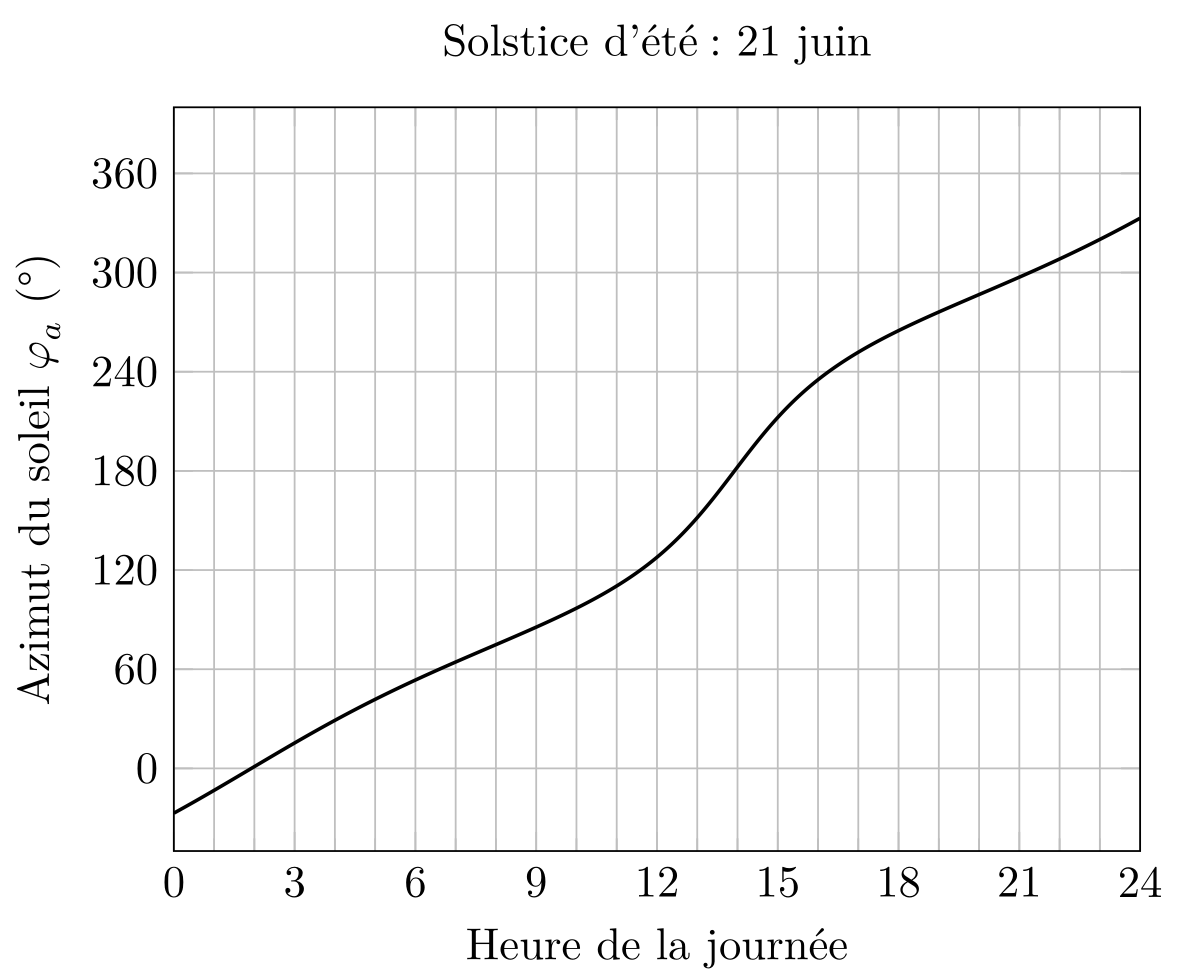
\includegraphics[width=0.7\linewidth]{img/fig03}
\end{center}
}{
\begin{center}
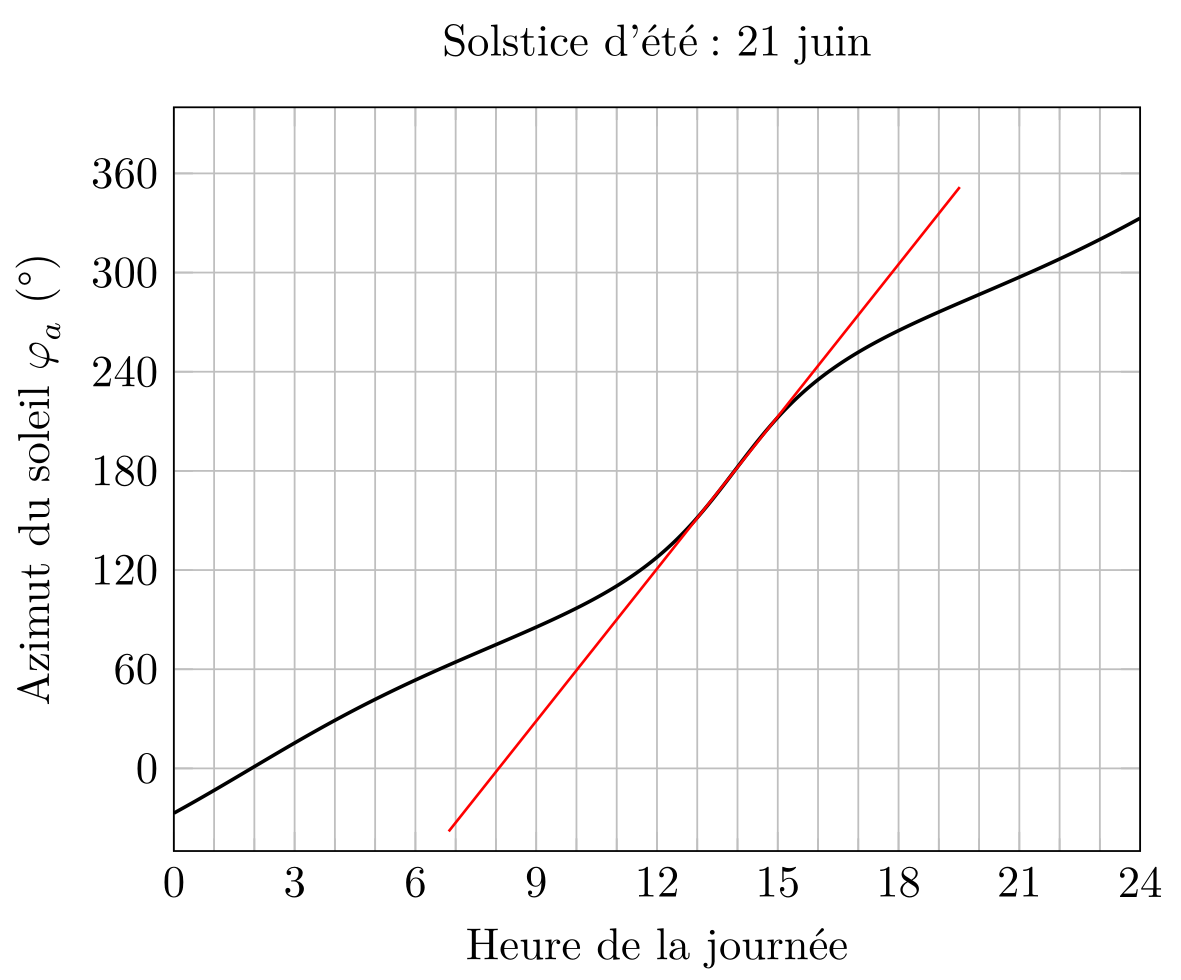
\includegraphics[width=0.7\linewidth]{img/fig03_cor}
\end{center}

La pente est $\dfrac{180-120}{14-12}=\dfrac{60}{2}=30^{\circ}\cdot h^{-1}$. Donc $\Omega_{max}=\dfrac{30}{3600}=\dfrac{1}{120}=0.008^{\circ}\cdot s^{-1}$.

Ainsi, en 15 min, il se déplace de $\dfrac{30}{4}=7.5^{\circ}$.
}

\reponse{4}{}{
$\varphi_{a\ max}=\left(d_{cste}+d_{acc}\right)\cdot\Omega_{max}$

$d_{cste}=\dfrac{\varphi_{a\ max}}{\Omega_{max}}-d_{acc}$
}

\reponse{6}{}{
$d_{totale}=d_{cste}+d_{acc}+d_{dec}=\dfrac{7.5}{0.18}+3s=\dfrac{2.5}{0.06}+3=\dfrac{0.1}{0.06}+\dfrac{2.4}{0.06}+3\approx 44,6s$.
}

\reponse{7}{}{
On lit sur la figure que $V_{dep}=\dfrac{3,651}{49}\approx 0,073m\cdot s^{-1}$. Donc $\omega_{dep}=\dfrac{0,073}{22,75}=10^{-3}\dfrac{73}{22,75}=10^{-3}(3+\dfrac{4,75}{22,75})\approx 3,2\cdot 10^{-3}rad\cdot s^{-1}\approx 3,2\cdot\dfrac{180}{\pi}\cdot 10^{-3}\ ^{\circ}\cdot s^{-1}\approx 0,19\cdot 10^{-3}\ ^{\circ}\cdot s^{-1}>0,18\ ^{\circ}\cdot s^{-1}$. L'exigence \og Id 1.1 \fg\ n'est pas respectée.

$49s<1min$ donc l'exigence \og Id 1.2 \fg\ est bien respectée.
}

\reponse{6}{}{
L'écart de position entre les deux voiles est de $3,651-3,633=0,018m>0,015m$. L'exigence \og Id 1.5 \fg\ n'est pas respectée. La perturbation du vent influence la précision du système.
}

\newpage

\reponse{0}{
\begin{center}
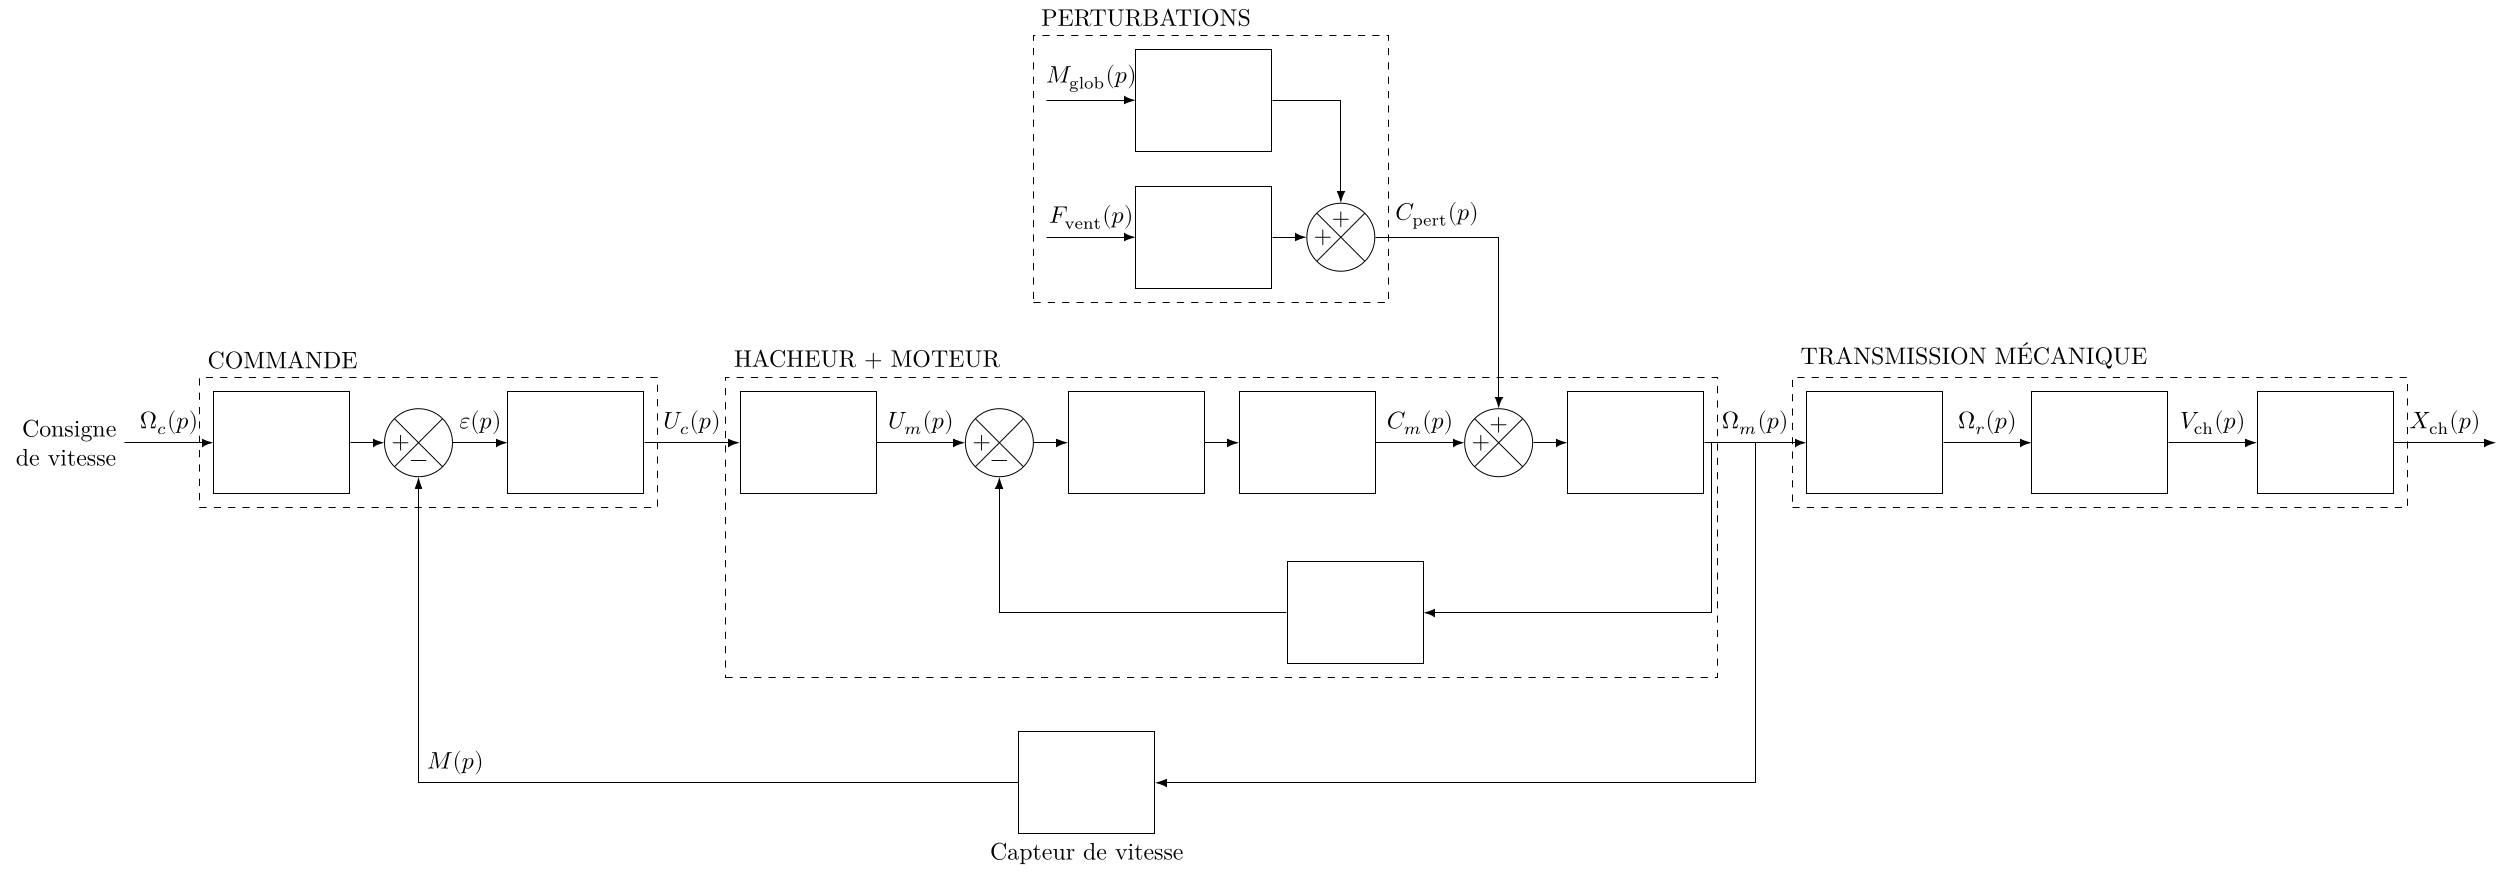
\includegraphics[width=1.3\linewidth,angle=90]{img/DR02}
\end{center}
}{
\begin{center}
\vspace{-2cm}
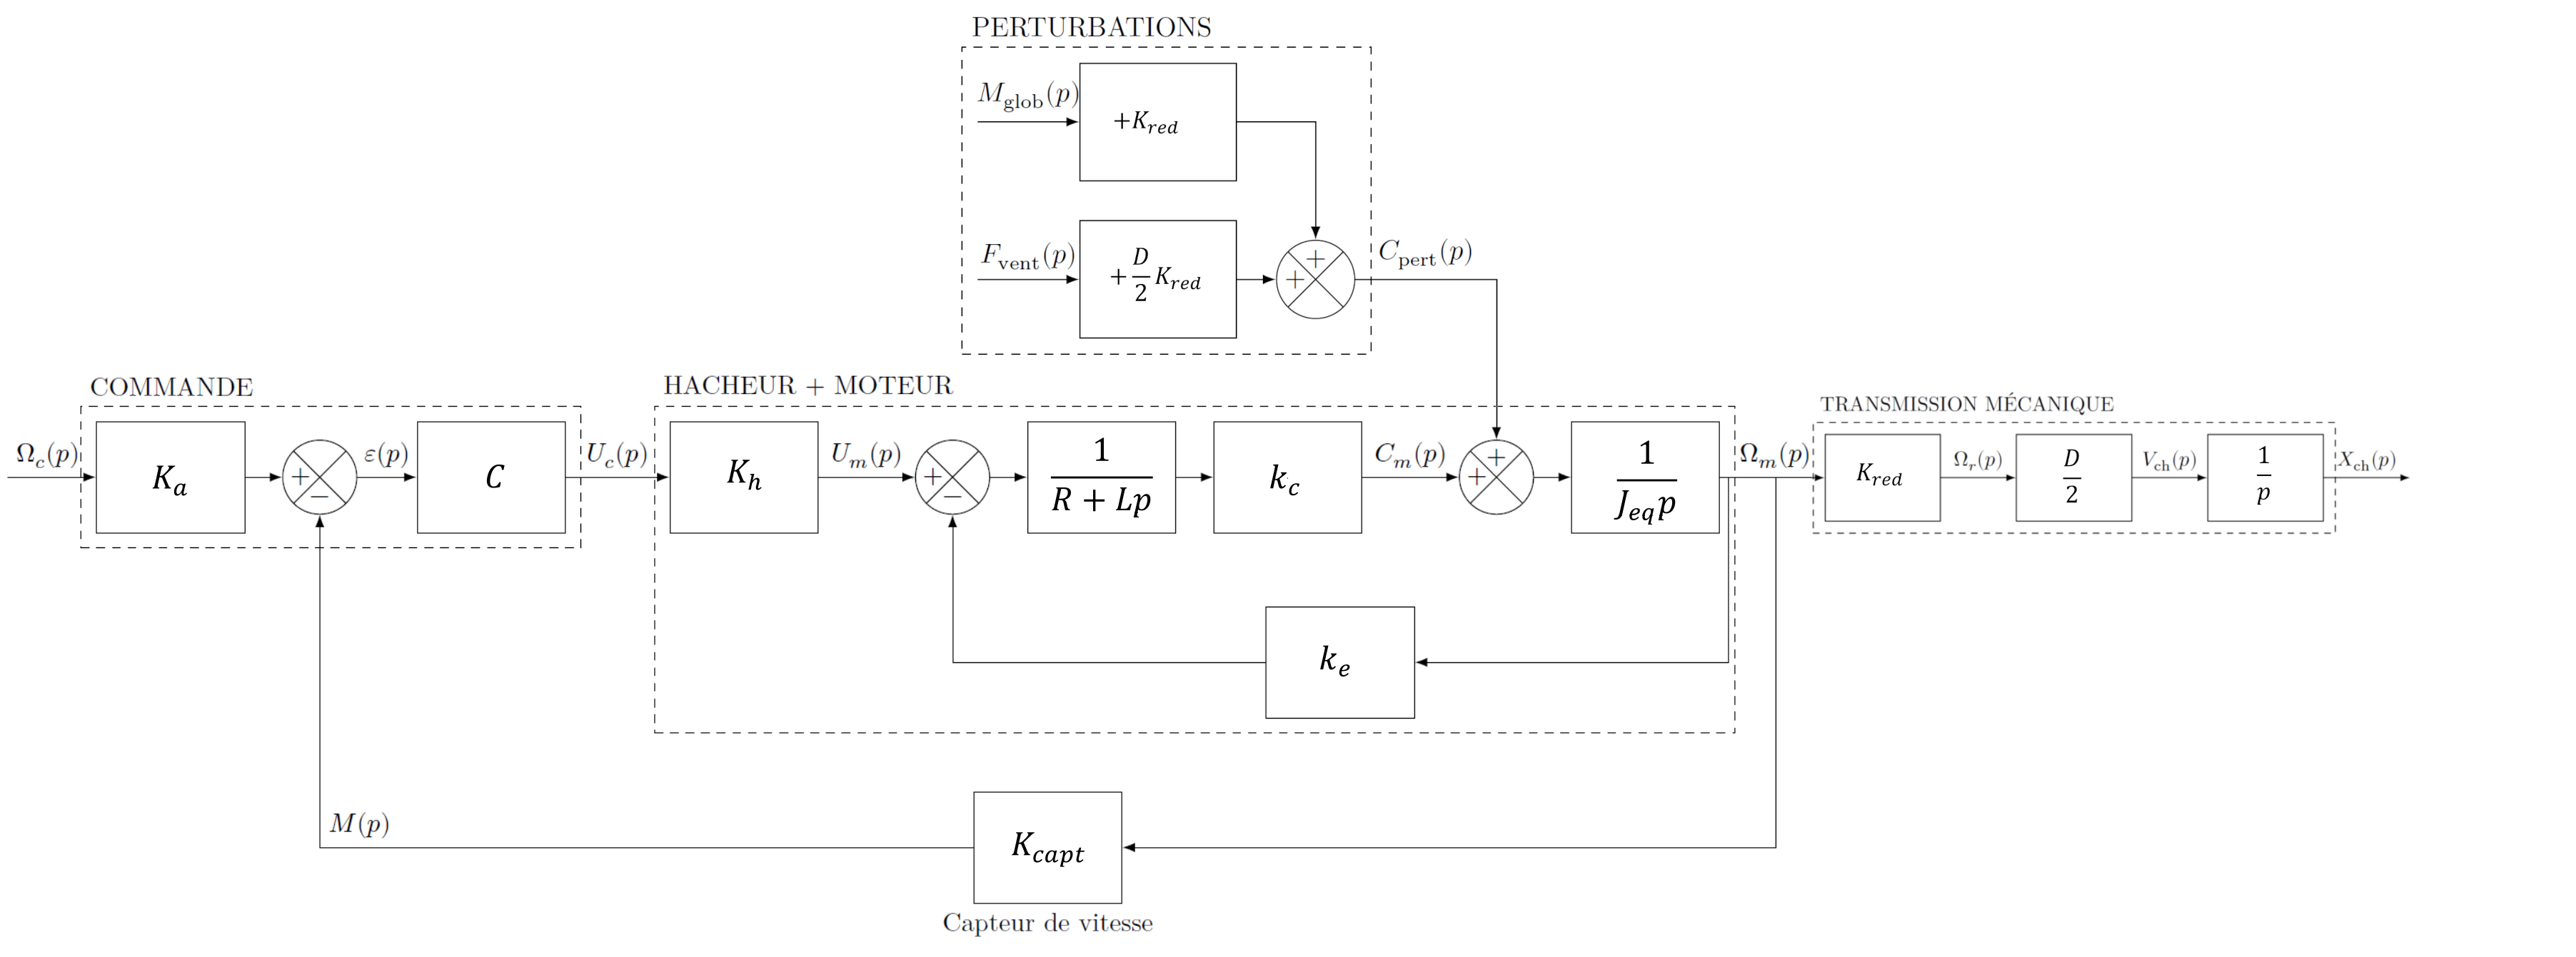
\includegraphics[width=1.5\linewidth,angle=90]{img/DR02_cor}
\end{center}
}

\newpage

\reponse{3}{
\begin{tabular}{|p{0.3\textwidth}|p{0.3\textwidth}|p{0.3\textwidth}|}
\hline
Grandeur & Unité & Unité S.I. de base \\
\hline
$\Omega_c(p)$ & $rad\cdot s^{-1}$ & $s^{-1}$ \\ 
\hline
$\varepsilon(p)$ & & \\
\hline
$U_c(p)$ & & \\
\hline
$C_m(p)$ & & \\
\hline
\end{tabular}
}{
\begin{tabular}{|p{0.3\textwidth}|p{0.3\textwidth}|p{0.3\textwidth}|}
\hline
Grandeur & Unité & Unité S.I. de base \\
\hline
$\Omega_c(p)$ & $rad\cdot s^{-1}$ & $s^{-1}$ \\ 
\hline
$\varepsilon(p)$ & $V$ & $kg\cdot m^2\cdot s^{-3}\cdot A^{-1}$ \\
\hline
$U_c(p)$ & $V$ & $kg\cdot m^2\cdot s^{-3}\cdot A^{-1}$ \\
\hline
$C_m(p)$ & $N\cdot m$ & $kg\cdot m^2\cdot s^{-2}$ \\
\hline
\end{tabular}
}

\reponse{3}{}{
$\varepsilon(t)=0\Leftrightarrow\varepsilon(p)=0\Leftrightarrow\Omega_c(p)\cdot K_a-\Omega_m(p)\cdot K_{capt}=0$.

Or $\omega_c(t)=\omega_m(t)\Leftrightarrow\Omega_c(p)=\Omega_m(p)\Rightarrow\Omega_c(p)\cdot(K_a-K_{capt})=0\Rightarrow K_a=K_{capt}$.}

\reponse{3}{}{
$H_{BO}=K_{capt}\cdot C\cdot K_h\cdot\dfrac{\dfrac{1}{k_e}}{1+\dfrac{R\cdot J_{eq}}{k_e\cdot k_t}\cdot p+\dfrac{L\cdot J_{eq}}{k_e\cdot k_t}\cdot p^2}$
}

\reponse{5}{}{
$H_{BF}=K_a\dfrac{C\cdot K_h\cdot\dfrac{\dfrac{1}{k_e}}{1+\dfrac{R\cdot J_{eq}}{k_e\cdot k_t}\cdot p+\dfrac{L\cdot J_{eq}}{k_e\cdot k_t}\cdot p^2}}{1+K_{capt}\cdot C\cdot K_h\cdot\dfrac{\dfrac{1}{k_e}}{1+\dfrac{R\cdot J_{eq}}{k_e\cdot k_t}\cdot p+\dfrac{L\cdot J_{eq}}{k_e\cdot k_t}\cdot p^2}}$

$H_{BF}=\dfrac{K_a\cdot C\cdot K_h\cdot\dfrac{1}{k_e}}{1+\dfrac{R\cdot J_{eq}}{k_e\cdot k_t}\cdot p+\dfrac{L\cdot J_{eq}}{k_e\cdot k_t}\cdot p^2+K_{capt}\cdot C\cdot K_h\cdot\dfrac{1}{k_e}}$

$H_{BF}=\dfrac{\dfrac{K_a\cdot C\cdot K_h}{k_e+K_{capt}\cdot C\cdot K_h}}{1+\dfrac{R\cdot J_{eq}}{(k_e\cdot k_t+K_{capt}\cdot C\cdot K_h\cdot k_t)}\cdot p+\dfrac{L\cdot J_{eq}}{(k_e\cdot k_t+K_{capt}\cdot C\cdot K_h\cdot k_t)}\cdot p^2}$
}

\reponse{5}{}{
$\varepsilon_s=\lim\limits_{p\rightarrow 0}p\cdot (1-H_{BF}(p))\cdot \dfrac{1}{p}=1-\dfrac{K_a\cdot C\cdot K_h}{k_e+K_{capt}\cdot C\cdot K_h}=\dfrac{k_e}{k_e+K_{capt}\cdot C\cdot K_h}$
}

\reponse{8}{}{
$\left\{\begin{array}{l}
\varepsilon(p)=-M(p)=-\Omega_m(p)\cdot K_{capt}\\
U_m(p)=K_h\cdot C\cdot \varepsilon(p)\\
C_m(p)=k_c\cdot \dfrac{1}{R+L\cdot p}\cdot \left(U_m(p)-k_e\cdot \Omega_m(p)\right)\\
\Omega_m(p)=\dfrac{1}{J_{eq}\cdot p}\cdot \left(C_m(p)+C_{pert}(p)\right)\\
\end{array}\right.$

$H_r(p)=\dfrac{\Omega_m(p)}{C_{pert}(p)}$

$\Omega_m(p)=\dfrac{1}{J_{eq}\cdot p}\cdot \left(k_c\cdot \dfrac{1}{R+L\cdot p}\cdot \left(-K_h\cdot C\cdot \Omega_m(p)\cdot K_{capt}-k_e\cdot \Omega_m(p)\right)+C_{pert}(p)\right)$

$\Omega_m(p)=-\dfrac{1}{J_{eq}\cdot p}\cdot k_c\cdot \dfrac{1}{R+L\cdot p}\cdot \left(K_h\cdot C\cdot K_{capt}+k_e\right)\cdot \Omega_m(p)+\dfrac{C_{pert}(p)}{J_{eq}}$

$\Omega_m(p)\left[1+\dfrac{1}{J_{eq}\cdot p}\cdot k_c\cdot \dfrac{1}{R+L\cdot p}\cdot \left(K_h\cdot C\cdot K_{capt}+k_e\right)\right]=\dfrac{C_{pert}(p)}{J_{eq}\cdot p}$

$H_r(p)=\dfrac{\dfrac{1}{J_{eq}\cdot p}}{1+\dfrac{1}{J_{eq}\cdot p}\cdot k_c\cdot \dfrac{1}{R+L\cdot p}\cdot \left(K_h\cdot C\cdot K_{capt}+k_e\right)}$

$H_r(p)=\dfrac{R+L\cdot p}{R\cdot J_{eq}\cdot p+L\cdot J_{eq}\cdot p^2+\cdot k_c\cdot \left(K_h\cdot C\cdot K_{capt}+k_e\right)}$

Avec $C=1$

$H_r(p)=\dfrac{\dfrac{R}{k_c\cdot \left(K_h\cdot K_{capt}+k_e\right)}\cdot \left(1+\dfrac{L}{R}\cdot p\right)}{1+\dfrac{R\cdot J_{eq}}{k_c\cdot \left(K_h\cdot K_{capt}+k_e\right)}\cdot p+\dfrac{L\cdot J_{eq}}{k_c\cdot \left(K_h\cdot K_{capt}+k_e\right)}\cdot p^2}$

$\left\{\begin{array}{l}
\alpha=\dfrac{-R}{k_c\cdot \left(K_h\cdot K_{capt}+k_e\right)}\\
\tau=\dfrac{L}{R}\\
\gamma=\dfrac{R\cdot J_{eq}}{k_c\cdot \left(K_h\cdot K_{capt}+k_e\right)}\\
\delta=\dfrac{L\cdot J_{eq}}{k_c\cdot \left(K_h\cdot K_{capt}+k_e\right)}
\end{array}\right.$}

\reponse{8}{}{
$H_r(p)=\dfrac{1}{25+5\cdot 10^{-2}\cdot p+2\cdot 10^{-4}\cdot p^2}$

$\Omega_m(p)=\dfrac{1}{25+5\cdot 10^{-2}\cdot p+2\cdot 10^{-4}\cdot p^2}\cdot \dfrac{C_0}{p}$

$\lim\limits_{t\rightarrow+\infty}\omega_m(t)=\lim\limits_{p\rightarrow 0}p\cdot \Omega_m(p)=\dfrac{C_0}{25}$
}

\reponse{8}{}{
$H_{BO}(p)=\dfrac{1.05}{1+5\cdot 10^{-3}\cdot p+2\cdot 1.9\cdot 10^{-5}\cdot p^2}\approx \dfrac{1}{1+5\cdot 10^{-3}\cdot p+2\cdot 10^{-5}\cdot p^2}$

$\omega_0=\sqrt{\dfrac{10^5}{2}}=\sqrt{5\cdot 10^4}=10^2\cdot \sqrt{5}\approx 220rad\cdot s^{-1}$

$K=1.05$

$\xi=\dfrac{\omega_0}{2}\cdot 5\cdot 10^{-3}=\dfrac{\sqrt{5}}{4}\approx \dfrac{2.2}{5}\approx 0.5$
}

\reponse{3}{
\begin{center}
 \def\svgwidth{.8\linewidth}
    \input{img/DR03.pdf_tex}
\end{center}
}{
\begin{center}
 \def\svgwidth{.8\linewidth}
    \input{img/DR03_cor.pdf_tex}
\end{center}
}


\reponse{7}{}{
$\dfrac{\left|H_{max}\right|}{\left|H(0)\right|}=\dfrac{1}{2\cdot\xi\cdot\sqrt{1-\xi^2}}$

$\left|H_{max}\right|=\dfrac{1}{2\cdot 0.5\cdot\sqrt{1-0.5^2}}=\dfrac{1}{\sqrt{0.75}}=\dfrac{1}{0.5\cdot \sqrt{3}}\approx \dfrac{2}{1.7}\approx 1.16$
}

\reponse{7}{}{
On remarque que lors d’un déplacement, l’écart relatif entre les deux voiles est inférieur à 1 mm, ce qui est conforme au cahier des charges. Cependant, le sujet insiste sur le fait qu'il y a plusieurs cycles par jour et chaque cycle peut augmenter l'écart. Donc, il paraît judicieux de mettre en place une solution de synchronisation.
}

\reponse{7}{}{
$u_{c\ 2}(t)=F_{corr}\left(m_1-2\cdot m_2+\omega_c\cdot K_{adapt}\right)$

En cas de vitesse identique entre les deux moteurs, $m_1=m_2$, le second sommateur du moteur 2 n'a aucune
influence et la commande du moteur 2 n’est donc pas modifiée. On retrouve celle de la fin de la section III.

Si la vitesse de rotation du second moteur est plus faible, alors on aura $m_1>m_2$ et le signal de sortie du second sommateur sera augmenté, ce qui va monter la consigne du moteur 2. La vitesse du moteur 2 va alors augmenter jusqu’à redevenir égal à celle du moteur 1.

Si la vitesse de rotation du second moteur est plus grande, alors on aura $m_1<m_2$ et le signal de sortie du second sommateur sera diminué, ce qui va baisser la consigne du moteur 2. La vitesse du moteur 2 va alors diminuer jusqu’à redevenir égal à celle du moteur 1.

Le schéma de synchronisation proposé permet de corriger correctement le système en cas d’écart entre les
vitesses des deux moteurs.
}

\end{document}
